\documentclass[11pt,a4paper]{report}

\usepackage{multicol}
\usepackage{graphicx}
\usepackage[left=2cm, right=2cm, top=2cm, bottom=4cm]{geometry}

%%%%%%%%%%%%%%%%%%%%%%%%%%%%%%%%%%%%%%%%%%%%

\begin{document}

\title{\textbf{Analysis of the dataset\\\textit{Credit Card Default}}}
\author{Gaspare Ferraro (520549)\\Javad	Khalili (546677)\\Mario	Matovic (583449)}
\date{\today}

% Definition of \maketitle
\makeatletter
    \begin{titlepage}
        \begin{center}
            { . }\\[20ex]
            {\huge \bfseries  \@title }\\[10ex] 
            {\LARGE  \@author}\\[10ex] 
            {\large \@date}\\[45ex]
            
            \noindent
            \begin{minipage}[c]{0.25\linewidth}
              
\includegraphics[width=0.9\linewidth]{img/cherubino}\\[4ex]
            \end{minipage} % no space if you would like to put them side by side
            \begin{minipage}[c]{0.7\linewidth}
              University of Pisa\\
              Exam: Data Mining\\
              Year: 2018/2019\\
              Instructors: Dino Pedreschi, Anna Monreale, Riccardo Guidotti
            \end{minipage}

        \end{center}
    \end{titlepage}
\makeatother
\thispagestyle{empty}
\newpage

\tableofcontents

%S\renewcommand{\cleardoublepage}{}
%\renewcommand{\clearpage}{}

%%%%%%%%%%%%%%%%%%%%%%%%%%%%%%%%%%%%%%%%%%%%%%%%%%%%%%%%%%%%%%%%%%%%%%%%%%%%%%%
\chapter{Introduction}


This research aimed at the case of customers default payments in Taiwan and compares the predictive accuracy of probability of default among six data mining methods. From the perspective of risk management the binary result of classification will valuable for identifying credible or not credible clients.


TEST TEST TEST TEST TEST TEST TEST TEST TEST TEST TEST TEST TEST TEST TEST TEST TEST TEST TEST TEST TEST TEST TEST TEST TEST TEST TEST TEST TEST TEST TEST TEST TEST TEST 

%%%%%%%%%%%%%%%%%%%%%%%%%%%%%%%%%%%%%%%%%%%%%%%%%%%%%%%%%%%%%%%%%%%%%%%%%%%%%%%
\chapter{Data Understanding}

The dataset is composed by 10000 records. Each record represents a customer, described by $24$ different attributes.

\section{Data semantics, distribution and statistics}

In this section we will analyze, for each attribute, its semantic and we will show interesting statistic and plot.
We have used.

We have discretized the continuous attribute by the natural binning method. For these attributes, mode has also been reported.

%%%%%%%%%%%%%%%%%%%%%%%%%%%%%%%%%%%%%%%%%%%%%%%%%%%%%%
\smallskip
\begin{figure}[h]
  \begin{minipage}[h]{.50\textwidth}
        {\Large \textbf{Sex}}
        
        Gender of the customer.
        
        A categorical attribute that can assume the values of \textit{male} ($3868$ of $10000$) or \textit{female} ($6032$ of $10000$). 
        
        Both of the gender values have a similar default rate ($25\%$ for males and $20\%$ for females).
  \end{minipage}
  \begin{minipage}[h]{.50\textwidth}
	  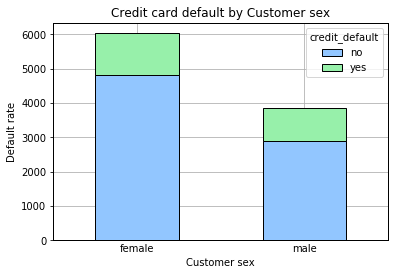
\includegraphics[width=.95\textwidth]{notebook/CardCardDefault_17_0}
  \end{minipage}
\end{figure}

%%%%%%%%%%%%%%%%%%%%%%%%%%%%%%%%%%%%%%%%%%%%%%%%%%%%%%
\smallskip
\begin{figure}[h]
  \begin{minipage}[h]{.45\textwidth}
	  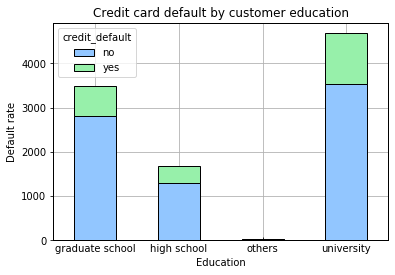
\includegraphics[width=.95\textwidth]{notebook/CardCardDefault_25_0}
  \end{minipage}
  \begin{minipage}[h]{.50\textwidth}
        {\Large \textbf{Education}}
        
        Qualification of the customer.
        
        A categorical attribute that can assume the values of 
        \textit{university} ($4685$ of $10000$),
        \textit{high school} ($1672$ of $10000$),
        \textit{graduate school} ($3480$ of $10000$) or
        \textit{others} ($36$ of $10000$).
        The default rate is again very similar for all the qualifications (around the $20\%$), except for the \textit{others} which is equal to $5\%$, but its number of records is very low to make any assumptions.
  \end{minipage}
\end{figure}
%%%%%%%%%%%%%%%%%%%%%%%%%%%%%%%%%%%%%%%%%%%%%%%%%%%%%%
\smallskip
\begin{figure}[h]
  \begin{minipage}[h]{.50\textwidth}
        {\Large \textbf{Status}}
        
        Marital status of the customer.
        
        A categorical attribute that can assume the values of 
        \textit{married} ($4685$ of $10000$),
        \textit{single} ($3757$ of $10000$) or
        \textit{other status} ($75$ of $10000$).
        
        The default rate is very similar for all the status (around the $25\%$).
  \end{minipage}
  \begin{minipage}[h]{.45\textwidth}
	  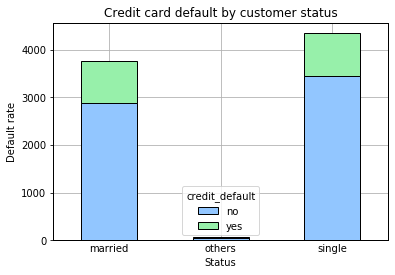
\includegraphics[width=.95\textwidth]{notebook/CardCardDefault_33_0}
  \end{minipage}
\end{figure}

%%%%%%%%%%%%%%%%%%%%%%%%%%%%%%%%%%%%%%%%%%%%%%%%%%%%%%
\smallskip
\begin{figure}[h]
  \begin{minipage}[h]{.45\textwidth}
	  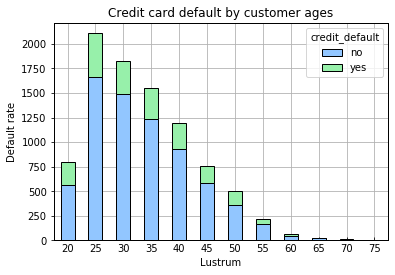
\includegraphics[width=.95\textwidth]{notebook/CardCardDefault_44_0}
  \end{minipage}
  \begin{minipage}[h]{.50\textwidth}
        {\Large \textbf{Age}}
        
        Age of the customer.
        
        An attribute that can assume integer values in $[21, 75]$ (this is due that in Taiwan the age of majority is $20$) and seems to be arranged according to a Gaussian distribution.
        
        The average is $35.5$ and the standard deviation is $9.22$, $50\%$ of the ages lie in $[28, 41]$.
        The bin with most elements is $25$.
        
        Again the default rate is similar for all the bins (around $25\%$).
  \end{minipage}
\end{figure}

%%%%%%%%%%%%%%%%%%%%%%%%%%%%%%%%%%%%%%%%%%%%%%%%%%%%%%
\smallskip

\begin{figure}[h]
  \begin{minipage}[h]{.50\textwidth}
        {\Large \textbf{Limit}}
        
        Limit of the credit card (expressed in NT dollar).
        
        It is the maximum amount the credit card company will let borrow on the account, 
        a continuous attribute that can assume values in $[10000, 780000]$ (all values are multiples of $10000$).
        
        The average is $167197$ and the standard deviation is $128975$, $50\%$ of the ages lie in $[50000, 240000]$. The bin with most elements is $50000$.
        
        The default rate in this case is very different for each bin as it decrease with the limit: the first bin has a default rate of $38\%$, the second one of $26\%$ and around $10\%$ for the higher bins.
        
  \end{minipage}
  \begin{minipage}[h]{.45\textwidth}
    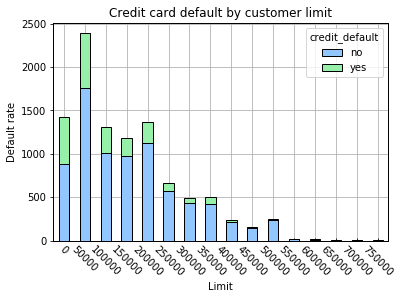
\includegraphics[width=.95\textwidth]{notebook/CardCardDefault_52_0}
  \end{minipage}

\end{figure}

\clearpage

%%%%%%%%%%%%%%%%%%%%%%%%%%%%%%%%%%%%%%%%%%%%%%%%%%%%%%
\smallskip
\begin{figure}[h]
  \begin{minipage}[h]{.40\textwidth}
        {\Large \textbf{Payment status}}
        

  \end{minipage}
  \begin{minipage}[h]{.60\textwidth}
    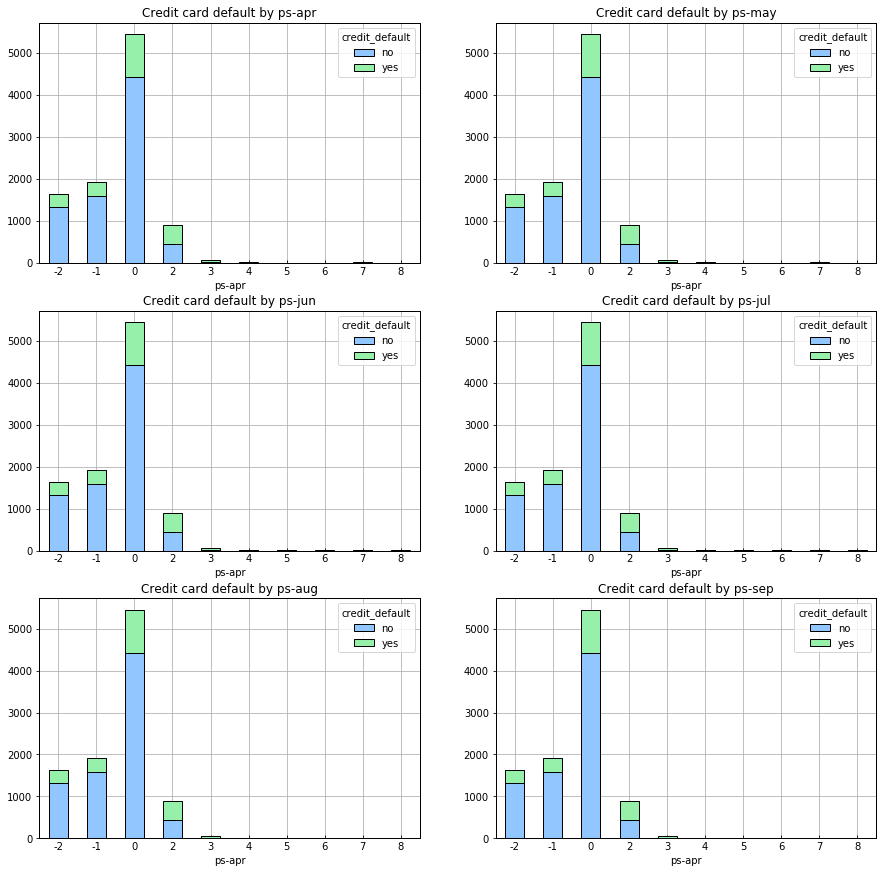
\includegraphics[width=.95\textwidth]{notebook/CardCardDefault_60_0}
  \end{minipage}
\end{figure}

%%%%%%%%%%%%%%%%%%%%%%%%%%%%%%%%%%%%%%%%%%%%%%%%%%%%%%
\smallskip
\begin{figure}[h]
  \begin{minipage}[h]{.40\textwidth}
        {\Large \textbf{Bill Amount}}
        

  \end{minipage}
  \begin{minipage}[h]{.60\textwidth}
    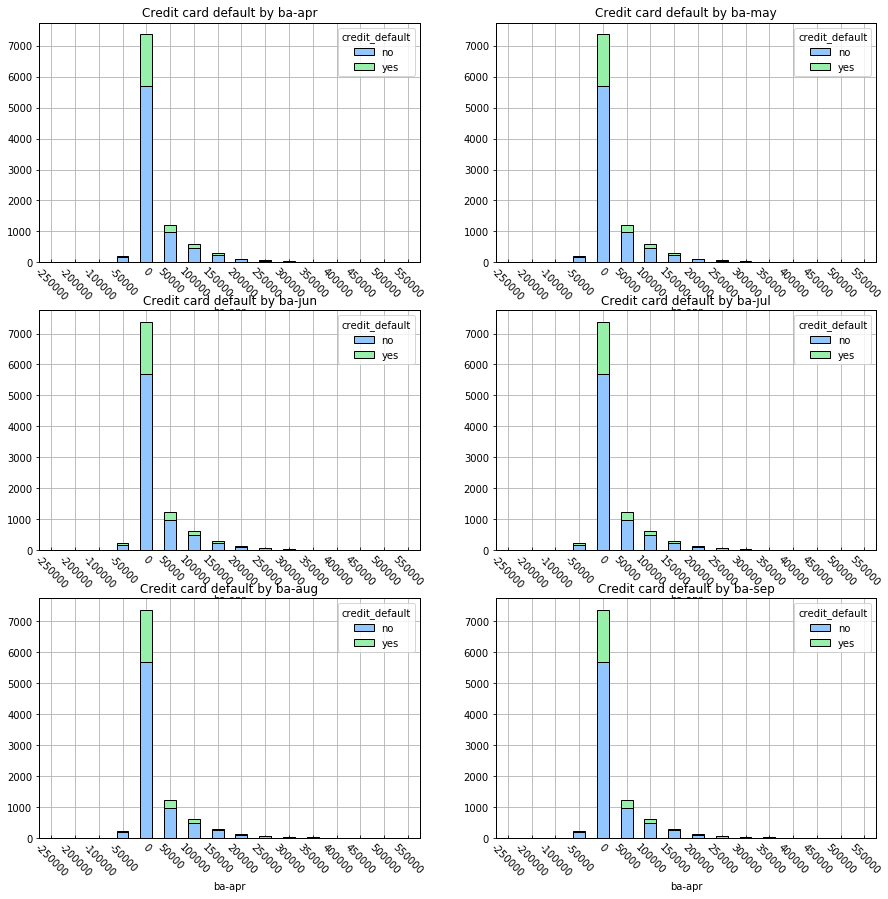
\includegraphics[width=.95\textwidth]{notebook/CardCardDefault_68_0}
  \end{minipage}
\end{figure}

%%%%%%%%%%%%%%%%%%%%%%%%%%%%%%%%%%%%%%%%%%%%%%%%%%%%%%
\smallskip
\begin{figure}[h]
  \begin{minipage}[h]{.40\textwidth}
        {\Large \textbf{Payment amount}}
        

  \end{minipage}
  \begin{minipage}[h]{.60\textwidth}
    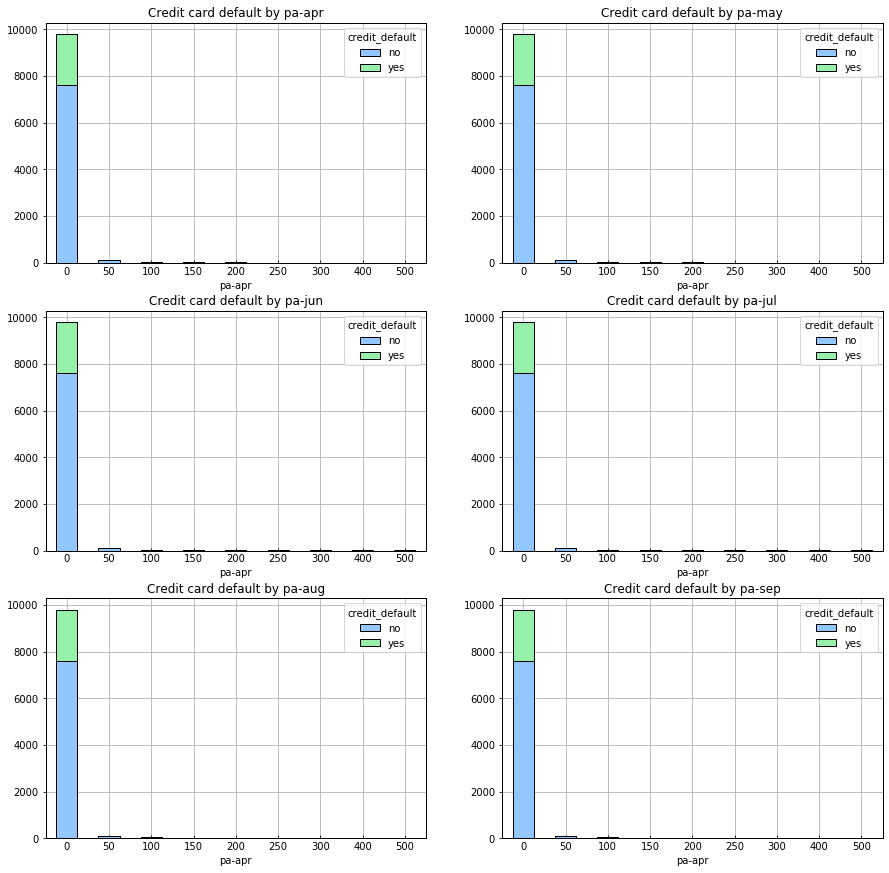
\includegraphics[width=.95\textwidth]{notebook/CardCardDefault_76_0}
  \end{minipage}
\end{figure}

%%%%%%%%%%%%%%%%%%%%%%%%%%%%%%%%%%%%%%%%%%%%%%%%%%%%%%%%%%%%%%%%%%%%%%%%%%%%%%%
\clearpage
\section{Assessing data quality}

Assessing data quality (missing values, outliers)

%%%%%%%%%%%%%%%%%%%%%%%%%%%%%%%%%%%%%%%%%%%%%%%%%%%%%%%%%%%%%%%%%%%%%%%%%%%%%%%
\section{Variables transformations}

modifica variabili
%%%%%%%%%%%%%%%%%%%%%%%%%%%%%%%%%%%%%%%%%%%%%%%%%%%%%%%%%%%%%%%%%%%%%%%%%%%%%%%
\clearpage

\section{Correlations and redundant variables}

\begin{figure}[h]
  \begin{minipage}[h]{.40\textwidth}
        Cose Cose cose Cose cose Cose cose
  \end{minipage}
  \begin{minipage}[h]{.60\textwidth}
    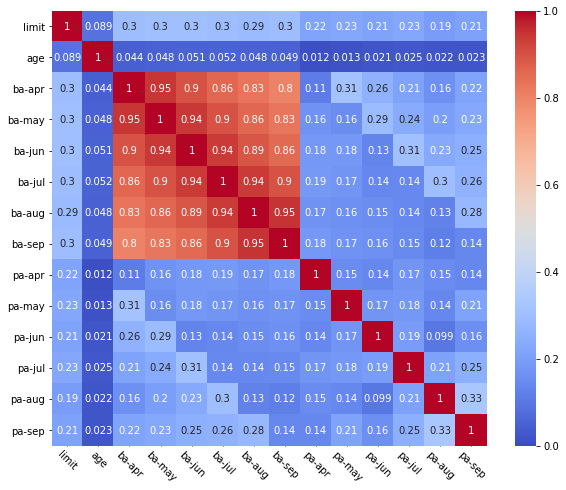
\includegraphics[width=.95\textwidth]{notebook/CardCardDefault_80_1}
  \end{minipage}
\end{figure}


\begin{figure}[h]
  \begin{minipage}[h]{.60\textwidth}
    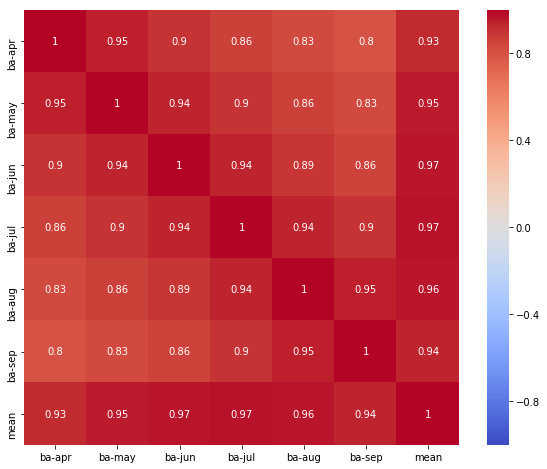
\includegraphics[width=.95\textwidth]{notebook/CardCardDefault_82_1}
  \end{minipage}
  \begin{minipage}[h]{.40\textwidth}
        Cose Cose cose Cose cose Cose cose
  \end{minipage}
\end{figure}
%%%%%%%%%%%%%%%%%%%%%%%%%%%%%%%%%%%%%%%%%%%%%%%%%%%%%%%%%%%%%%%%%%%%%%%%%%%%%%%
\chapter{Clustering}

\section{K-means}


\subsection{Choice of attributes and distance function}
\subsection{Choise of the best value of k}
\subsection{Cluster analysis}

\section{DBSCAN}
\subsection{Choice of attributes and distance function}
\subsection{Study of the clustering parameters}
\subsection{Characterization and interpretation of the obtained clusters}

\section{Hierarchical clustering}
\subsection{Choice of attributes and distance function}
\subsection{Discussion of dendograms using different algorithms}

\section{Evaluation of clustering approaches and comparison of the clustering obtained}

%%%%%%%%%%%%%%%%%%%%%%%%%%%%%%%%%%%%%%%%%%%%%%%%%%%%%%%%%%%%%%%%%%%%%%%%%%%%%%%
\chapter{Association Rules Mining}

\section{Frequent patterns extraction with different parameters}
\section{Discussion of the most interesting frequent patterns}
\section{Association rules extraction with different values of confidence}
\section{Discussion of the most interesting rules}
\section{Use the most meaningful rules to replace missing values}
\section{Use the most meaningful rules to predict credit card defaults}

%%%%%%%%%%%%%%%%%%%%%%%%%%%%%%%%%%%%%%%%%%%%%%%%%%%%%%%%%%%%%%%%%%%%%%%%%%%%%%%
\chapter{Classification}

\section{Choice of attributes for the decision trees}
\section{Decision trees interpretation and validation with test and training set}
\section{Discussion of the best prediction model}

%%%%%%%%%%%%%%%%%%%%%%%%%%%%%%%%%%%%%%%%%%%%%%%%%%%%%%%%%%%%%%%%%%%%%%%%%%%%%%%
\chapter{Conclusion}

%%%%%%%%%%%%%%%%%%%%%%%%%%%%%%%%%%%%%%%%%%%%%%%%%%%%%%%%%%%%%%%%%%%%%%%%%%%%%%%
\end{document}
